% !TEX root = ../document.tex
% !TeX spellcheck = pt_BR

\section{Introdução}
\label{sec:section1}

Doenças cardíacas são a principal causa de morte no Brasil e no mundo. De acordo com a Organização Mundial da Saúde \cite{Who04}, elas representam cerca de 30\% de todas as mortes mundiais. Em especial, a doença arterial coronariana é responsável por 12\% das mortes (7.2 milhões), tornando-a a principal causa de morte dentre as cardiopatias.

Esta doença provoca uma condição chamada isquemia do miocárdio, ou isquemia cardíaca, que é a falta de suprimento de sangue no músculo do coração. Eventos isquêmicos podem ser detectados em exames eletrocardiográficos (ECGs) pela análise de ondas características como o complexo QRS, o segmento ST e a onda T. Estes são conceitos criados para identificar etapas do ciclo cardíado humano, quando analisadas através do prisma da atividade elétrica do coração. A cada formato de onda dentro de um ciclo corresponde uma letra, começando pela letra `P', teminando em `T', e passando por `Q', `R' e `S'. ST é o segmento que se estende do fim da onda `S' até o início da onda `T'. A figura \ref{fig:normal_beat} mostra um exemplo de batida cardíaca normal obtida num exame eletrocardiográfico.

\begin{figure}[ht]
    \centering
    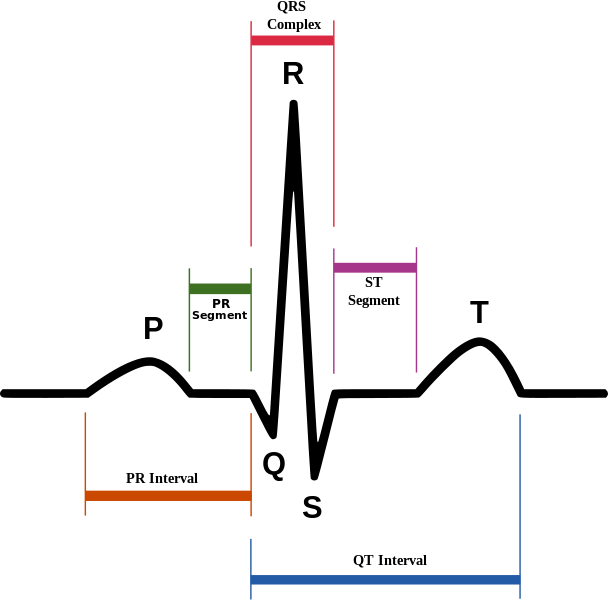
\includegraphics[width=0.6\textwidth]{figures/normal_beat.png}
    \caption{Batida cardíaca normal, e suas respectivas ondas características. Extraída de \cite{WikiSTSeg13}.}
    \label{fig:normal_beat}
\end{figure}

Batidas consideradas isquêmicas são distinguíveis no ECG porque alteram o formato das ondas características, sendo que a elevação ou depressão do segmento ST, bem como a inversão da onda T, são os principais critérios sobre os quais especialistas baseiam seus diagnósticos de isquemia cardíaca.

Visando acelerar o processo diagnóstico e permitir que pacientes recebam tratamento adequado o mais rapidamente possível, há um esforço da comunidade científica em desenvolver sistemas móveis capazes de detectar isquemia \emph{in loco} -- uso de PDAs (ver \cite{Couceiro08}), celulares (ver \cite{Varella11}), dispositívos implantáveis e não-duráveis (ver \cite{Rocha10}), microssistemas, entre outros. Sob esta perspectiva, tentaremos avaliar alguns métodos de detecção de isquemia já existentes no estado-da-arte, e selecionar aquele que apresenta melhor desempenho para ser empregado num sistema de monitoramento cardíaco móvel.

O trabalho está organizado da seguinte maneira: a seção \ref{sec:section1} dá uma visão geral dos métodos e de como eles foram selecionados; as seções \ref{sec:section2} a \ref{sec:section4} apresentam a implementação das primeiras etapas de cada um dos três algoritmos; por fim, a seção \ref{sec:section5} faz uma proposta de trabalho a ser desenvolvido para dar sequência ao presente estudo.

\subsection{Visão geral}

A escolha dos algoritmos é resultado de um estudo realizado por Guilherme Lima \cite{Lima01}, em que foram analisados diversos artigos científicos sobre a detecção de isquemia cardíaca em ECGs. Lima coletou dados de sensibilidade, preditividade positiva e acurácia, e selecionou 5 métodos como candidatos para uma investigação mais profunda, dos quais 3 estão sendo implementados e serão discutidos neste trabalho.

O primeiro método é o trabalho proposto por Rocha et al. \cite{Rocha10}, cuja estratégia de detecção envolve a caracterização do complexo QRS, do segmento ST e da onda T. Esta caracterização é baseada em uma análise tempo-frequencial do sinal de ECG e também na expansão em funções de Hermite (discutidas em detalhe na próxima seção). O algoritmo consiste em extrair dois conjuntos de características para cada batida, e usar um comitê de redes neurais para classificar uma batida em isquêmica ou não-isquêmica.

O segundo método é o de Mohebbi e Moghadam \cite{Mohebbi07}, em que a detecção é baseada na construção de um modelo (ou \emph{template}, em inglês) para o segmento ST de batidas normais. O algoritmo consiste basicamente em medir o quão diferente é um segmento ST em relação ao modelo, e fornecer essa diferença como entrada em uma rede neural. A rede então classificará a batida de que foi extraído o segmento em isquêmica ou não.

O terceiro método é o de Gopalakrishnan et al. \cite{Gopalak04}. Neste trabalho, uma estratégia semelhante à do primeiro método é adotada, usando funções de Hermite para aproximar o formato de uma batida cardíaca. Contudo, a formulação matemática aqui é maior, e os autores conseguem derivar um método de cálculo eficiente para as funções de Hermite, envolvendo matriz de Fourier e diversas propriedades da álgebra linear, como tridiagonalidade e comutatividade de matrizes, autovalores e autovetores, entre outras.
